\noindent Django is an open source web application framework written in python. It lets 
you build high-performing, elegant Web applications quickly. Django 
focuses on automating as much as possible. Django's primary goal is to 
ease the creation of complex, database-driven websites. Django 
emphasizes reusability and "pluggability" of components, rapid 
development, and the DRY principal. Python is used throughout, even 
for settings, files, and data models. Django also provides an optional
 administrative create, read, update and delete interface that is 
generated dynamically through introspection and configured via admin 
models.

Django takes it's name from the early jazz guitarist Django Reinhardt, 
a gypsy savant who managed to play dazzling and electrifying runs on 
his instrument even though two of the fingers on his left hand were 
paralyzed in an accident when he was young.

Thus it’s a fitting name for the framework. Django can do some very 
complex things with less code and a simpler execution than you’d expect. 
It doesn't take a heavy hand to build with Django. The framework does 
the repetitive work for you, allowing you to get a working website up 
quickly and easily.
\subsection{Features of Django}
\begin{itemize}
\item Clean URLs
\item Object- Relational Mapping
\item Loosely coupled components
\item Designer-friendly templates  
\item Cache framework 
\item MVC architecture
\item Jython support
\item DRY ( Don't Repeat Yourself)
\end{itemize}
\subsection{Installation of Django}
Installation of Django is very easy. To install Django version 1.4,
type the following commands:\\

	\$ wget http://www.djangoproject.com/download/1.4/tarball\\


	\$ tar xzvf Django-1.4.tar.gz\\


	\$ cd Django-1.4\\


	\$ sudo python setup.py install \\

\noindent This will install the django on your system.
 
\noindent \subsection{MTV} Django adopts the standard 
MVC (Model-View-Controller) design pattern. But instead, their naming 
convention is the MTV (Model-Template-View).
\begin{itemize}
\item {\bf{Model}} is an object relational mapping to your 
database schema. So each model is a class which represents a table in 
your database. Django models provide easy access to an underlying data 
storage mechanism, and can also encapsulate any core business logic, 
which must always remain in effect, regardless of which application is 
using it. Models exist independent of the rest of the system, and are 
designed to be used by any application that has access to them. In 
fact, the database manipulation methods that are available on model 
instances can be utilized even from the interactive interpreter, 
without loading a Web server or any application-specific logic.

\item {\bf{Template}} is simply HTML for your views. It also 
allows you to display different messages depending on whether or not a 
user is logged in. Templates are Django's provided way of generating 
text-based output, such as HTML or emails, where the people editing 
those documents may not have any experience with Python. Therefore, 
templates are designed to avoid using Python directly, instead favoring 
an extensible, easy-to-use custom language built just for Django.

\item {\bf{View}} could be a homepage or a page to display a 
user's information, for instance. A view accepts user input, including 
simple requests for information; behaves according to the application's 
interaction logic; and returns a display that is suitable for user's to 
access the data represented by models.
\end{itemize}
\subsection{Creating Prject in Django}
If this is your first time using Django, you'll have to take care of 
some initial setup. Namely, you'll need to auto-generate some code that 
establishes a Django project- a collection of settings for an instance 
of Django, including database configuration, Django-specific options 
and application-specific settings. From the command line, cd into a 
directory where you'd like to store your code, then run the command \\

	\$ django-admin.py startproject mysite \\

\noindent This will create a mysite directory in your current
directory.


\subsection{Development Server in Django}  Change into 
the outer mysite directory, if you haven't already, and run the command\\
	
	\$ python manage.py runserver\\

You'll see the following output on the command line:\\

\begin{figure}[h]
\centering 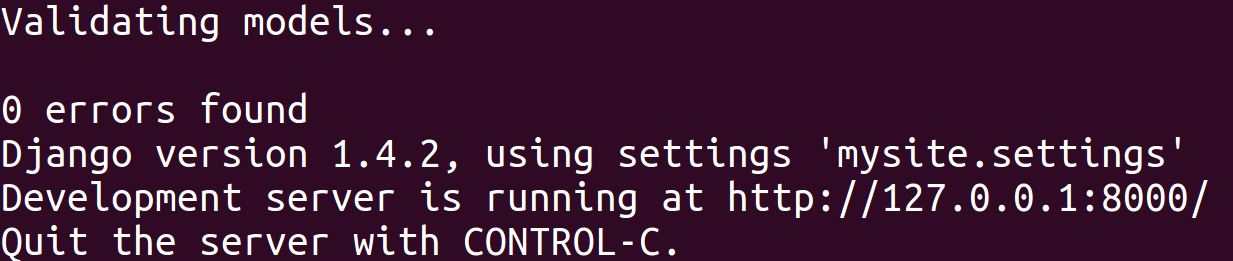
\includegraphics[scale=0.5]{images/out.jpg}
\caption{Output of runserver}
\end{figure}

\subsection{Database setup}
In this, we need to edit the settings.py file of the Project, that is the 
configuration file. It's a normal Python module with module-level 
variables representing Django settings. Change the following keys in 
the DATABASES 'default' item to match your database connection 
settings.
\begin{itemize}
\item ENGINE -- Either `django.db.backends.postgresql\_psycopg2', 
`django.db.backends.mysql',\\ `django.db.backends.sqlite3' or 
`django.db.backends.oracle'. Other backends are also available.
\item NAME -- The name of your database. If you're using SQLite, 
the database will be a file on your computer; in that case, NAME 
should be the full absolute path, including filename, of that file. If 
the file doesn't exist, it will automatically be created when you 
synchronize the database for the first time (see below). When specifying 
the path, always use forward slashes, even on Windows 
(e.g. C:/homes/user/mysite/sqlite3.db). 
\item USER -- Your database username (not used for SQLite).
\item PASSWORD -- Your database password (not used for SQLite).
\item HOST -- The host your database is on. Leave this as an empty 
string if your database server is on the same physical machine (not 
used for SQLite).
\end{itemize}

If you're new to databases, we recommend simply using SQLite by setting 
ENGINE to \\`django.db.backends.sqlite3' and NAME to the place where 
you'd like to store the database. SQLite is included as part of Python 
2.5 and later, so you won't need to install anything else to support 
your database.

While you're editing settings.py, set TIME\_ZONE to your time zone. The 
default value is the Central time zone in the U.S. (Chicago).

Also, note the INSTALLED\_APPS setting toward the bottom of the file. 
That holds the names of all Django applications that are activated in 
this Django instance. Apps can be used in multiple projects, and you 
can package and distribute them for use by others in their projects.

By default, INSTALLED\_APPS contain the following apps, all of which 
come with Django:
\begin{itemize}
\item django.contrib.auth -- An authentication system.
\item django.contrib.contenttypes -- A framework for content types.
\item django.contrib.sessions -- A session framework.
\item django.contrib.sites -- A framework for managing multiple sites 
with one Django installation.
\item django.contrib.messages -- A messaging framework.
\item django.contrib.staticfiles -- A framework for managing static 
files.
\end{itemize}

These applications are included by default as a convenience for the 
common case.

Each of these applications makes use of at least one database table, 
though, so we need to create the tables in the database before we can 
use them. To do that, run the following command:\\

	\$ python manage.py syncdb\\

The syncdb command looks at the INSTALLED\_APPS setting and creates 
any necessary database tables according to the database settings in 
your settings.py file. You'll see a message for each database table it 
creates, and you'll get a prompt asking you if you'd like to create a 
superuser account for the authentication system. Go ahead and do that.

\noindent \subsection{Django Applications used :}
\begin{itemize}
\item{\bf{Django Registation}}: It is an extensible 
user-registration application for Django. This is a fairly simple 
user-registration application for Django, designed to make allowing 
user signups as painless as possible. It requires a functional 
installation of Django 1.3 or newer, but has no other dependencies.\\
Django Registation module can be installed easily using :\\

\hspace{8pt} \$ pip install django-registration\\
 
\item{\bf{Django Tagging}}: This is a generic tagging 
application for Django, which allows association of a number of tags 
with any Model instance and makes retrieval of tags simple.

Django Registation module can be installed easily using :\\

\hspace{8pt} \$ pip install django-tagging\\
\end{itemize}
